\documentclass{article}
\usepackage{fancyhdr}
\usepackage{ctex}
\usepackage{listings}
\usepackage{graphicx}
\usepackage[a4paper, body={18cm,22cm}]{geometry}
\usepackage{amsmath,amssymb,amstext,wasysym,enumerate,graphicx}
\usepackage{float,abstract,booktabs,indentfirst,amsmath}
\usepackage{array}
\usepackage{booktabs}
\usepackage{multirow}
\usepackage{url}
\usepackage{diagbox}
\renewcommand\arraystretch{1.4}
\usepackage{indentfirst}
\setlength{\parindent}{2em}
\usepackage{enumitem}
\setmonofont{Consolas}
\usepackage{listings}
\usepackage{xcolor}
\usepackage{makecell}
\usepackage{tikz}
\usetikzlibrary{positioning, arrows.meta}
\setCJKmonofont{黑体}
\lstset{  
	% 基本设置  
	xleftmargin = 3em, xrightmargin = 3em, aboveskip = 1em,  
	backgroundcolor = \color{white},  
	basicstyle = \small\ttfamily,  
	rulesepcolor = \color{gray},  
	breaklines = true,  
	numbers = left,  
	numberstyle = \small,  
	numbersep = -14pt,  
	frame = shadowbox,  
	showspaces = false,  
	columns = fixed,  
	sensitive = true,  
	% VSCode 风格配色  
	keywordstyle = \color{blue!70!black}\bfseries,  
	emphstyle = \color{red!70!black}\bfseries, % 对于强调的词  
	emphstyle=[2]\color{purple!70!black}\bfseries, % 对于第二组强调的词  
	commentstyle = \color{green!60!black}, % 注释颜色  
	stringstyle = \color{orange!90!black}, % 字符串颜色更亮一些  
	morekeywords={ASSERT, int64\_t, uint32\_t},  
	moreemph={ASSERT, NULL},  
	moreemph=[2]{int64\_t, uint32\_t, tid\_t, uint8\_t, int16\_t, uint16\_t, int32\_t, size\_t, bool},  
	morecomment=[l][\color{green!60!black}]{+}, % 以+开头的注释  
}

%--------------------页眉--------------------%
\pagestyle{fancy}
\fancyhead[L]{}
\fancyhead[R]{}
\fancyhead[C]{华东师范大学软件工程学院实验报告}
\fancyfoot[C]{-\thepage-}
\renewcommand{\headrulewidth}{1.5pt}
%--------------------标题--------------------%
\begin{document}
\begin{center}
	{\Large{\textbf{\heiti 实验六——系统调用}}}
	\begin{table}[H]
		\centering
		\begin{tabular}{p{2cm}p{4cm}<{\centering}p{1cm}p{2cm}p{6cm}<{\centering}}
			课程名称:    & 操作系统实践 & \quad & 指导教师:    & 张民
			\\ \cline{2-2} \cline{5-5}
			姓\qquad 名: & 王海生    & \quad & 学\qquad 号: & 10235101559         \\ \cline{2-2} \cline{5-5}
			实验编号:    & 实验六 & \quad & 实验名称:    & 系统调用
			\\ \cline{2-2} \cline{5-5}
		\end{tabular}
	\end{table}
	
	% 添加新行并居中
	%\vspace{1em} % 可选:添加垂直间距
	\textbf{代码仓库:}\url{https://github.com/Hanson-Wang-chn/ECNU-Operating-System-WHS.git}
\end{center}
\rule{\textwidth}{1pt}

\tableofcontents

%--------------------正文--------------------%
\section{实验目的}

\begin{enumerate}
	\item 完成系统调用,使得\texttt{make check}通过\texttt{create}、\texttt{open}、\texttt{close}、\texttt{read}相关测试。
	\item 完成实验报告并提交。无需提交代码文件,只需要提交报告的\texttt{pdf}即可。在报告中介绍对系统调用的分析过程,展示代码中需要修改的地方,解释修改的含义,和运行结果。
	\item 可选扩展任务(不强求):继续完成其他系统调用,通过\texttt{make check}中其他的测试点。相关内容也写在实验报告中。
\end{enumerate}

\normalsize

\section{实验内容与设计思想}

本次实验的主要任务是实现\texttt{Pintos}操作系统中的系统调用功能。系统调用是用户程序与操作系统内核之间的接口,用户程序通过系统调用请求内核提供服务,如文件操作、进程控制等。实验的核心目标是实现一系列系统调用,并通过\texttt{Pintos}提供的测试用例验证其正确性。

实验内容主要包括以下几个方面:
\begin{enumerate}
	\item \textbf{系统调用的基本框架}:首先需要理解\texttt{Pintos}中系统调用的处理流程,包括如何从用户态切换到内核态,如何传递参数,以及如何返回结果。通过修改\texttt{syscall.c}文件,实现系统调用的基本框架。
	
	\item \textbf{进程相关的系统调用}:实现\texttt{halt}、\texttt{exit}、\texttt{exec}、\texttt{wait}等进程控制系统调用。这些系统调用涉及到进程的创建、终止、等待等操作,需要仔细处理进程间的同步问题,确保父子进程的正确通信。
	
	\item \textbf{文件相关的系统调用}:实现\texttt{create}、\texttt{remove}、\texttt{open}、\texttt{close}、\texttt{read}、\texttt{write}等文件操作系统调用。这些系统调用涉及到文件的创建、删除、打开、关闭、读写等操作,需要注意文件系统的线程安全性,确保多个进程对文件的并发访问不会导致数据不一致。
	
	\item \textbf{内存访问检查}:在系统调用中,用户程序可能会传递非法地址,因此需要实现对用户内存地址的检查,确保用户程序只能访问其合法的内存空间。通过\texttt{check\_ptr}函数对用户传递的指针进行检查,防止非法访问。
	
	\item \textbf{扩展任务}:在完成基本任务后,还可以进一步实现\texttt{seek}、\texttt{tell}等文件操作系统调用,并通过\texttt{make check}中的更多测试用例,验证系统的完整性和稳定性。
\end{enumerate}

在实验过程中,我逐步理解了系统调用的实现机制,并通过调试和测试,解决了进程同步、文件系统线程安全等问题。最终,\textbf{所有的测试用例均通过}。

\section{使用环境}

\subsection{主机系统配置}

本次实验的主机系统环境如下表所示:

\begin{center}
	\begin{tabular}{| >{\centering\arraybackslash}m{3cm} | >{\centering\arraybackslash}m{7cm} |}    
		\hline  
		\textbf{项目名称} & \textbf{详细信息} \\
		\hline  
		操作系统 & macOS Sequoia 15.2 \\  
		\hline  
		系统类型 & 64位操作系统,基于ARM的处理器 \\  
		\hline
		CPU & Apple M1 Pro \\  
		\hline 
		GPU & Apple M1 Pro\\  
		\hline 
		内存 & 32GB 统一内存 \\  
		\hline 
		磁盘 & 512GB SSD \\  
		\hline 		
	\end{tabular}
\end{center}

\subsection{Docker配置}

在官网下载并安装后,Docker容器正常运行,如下图所示:

\begin{figure}[H]
	\centering
	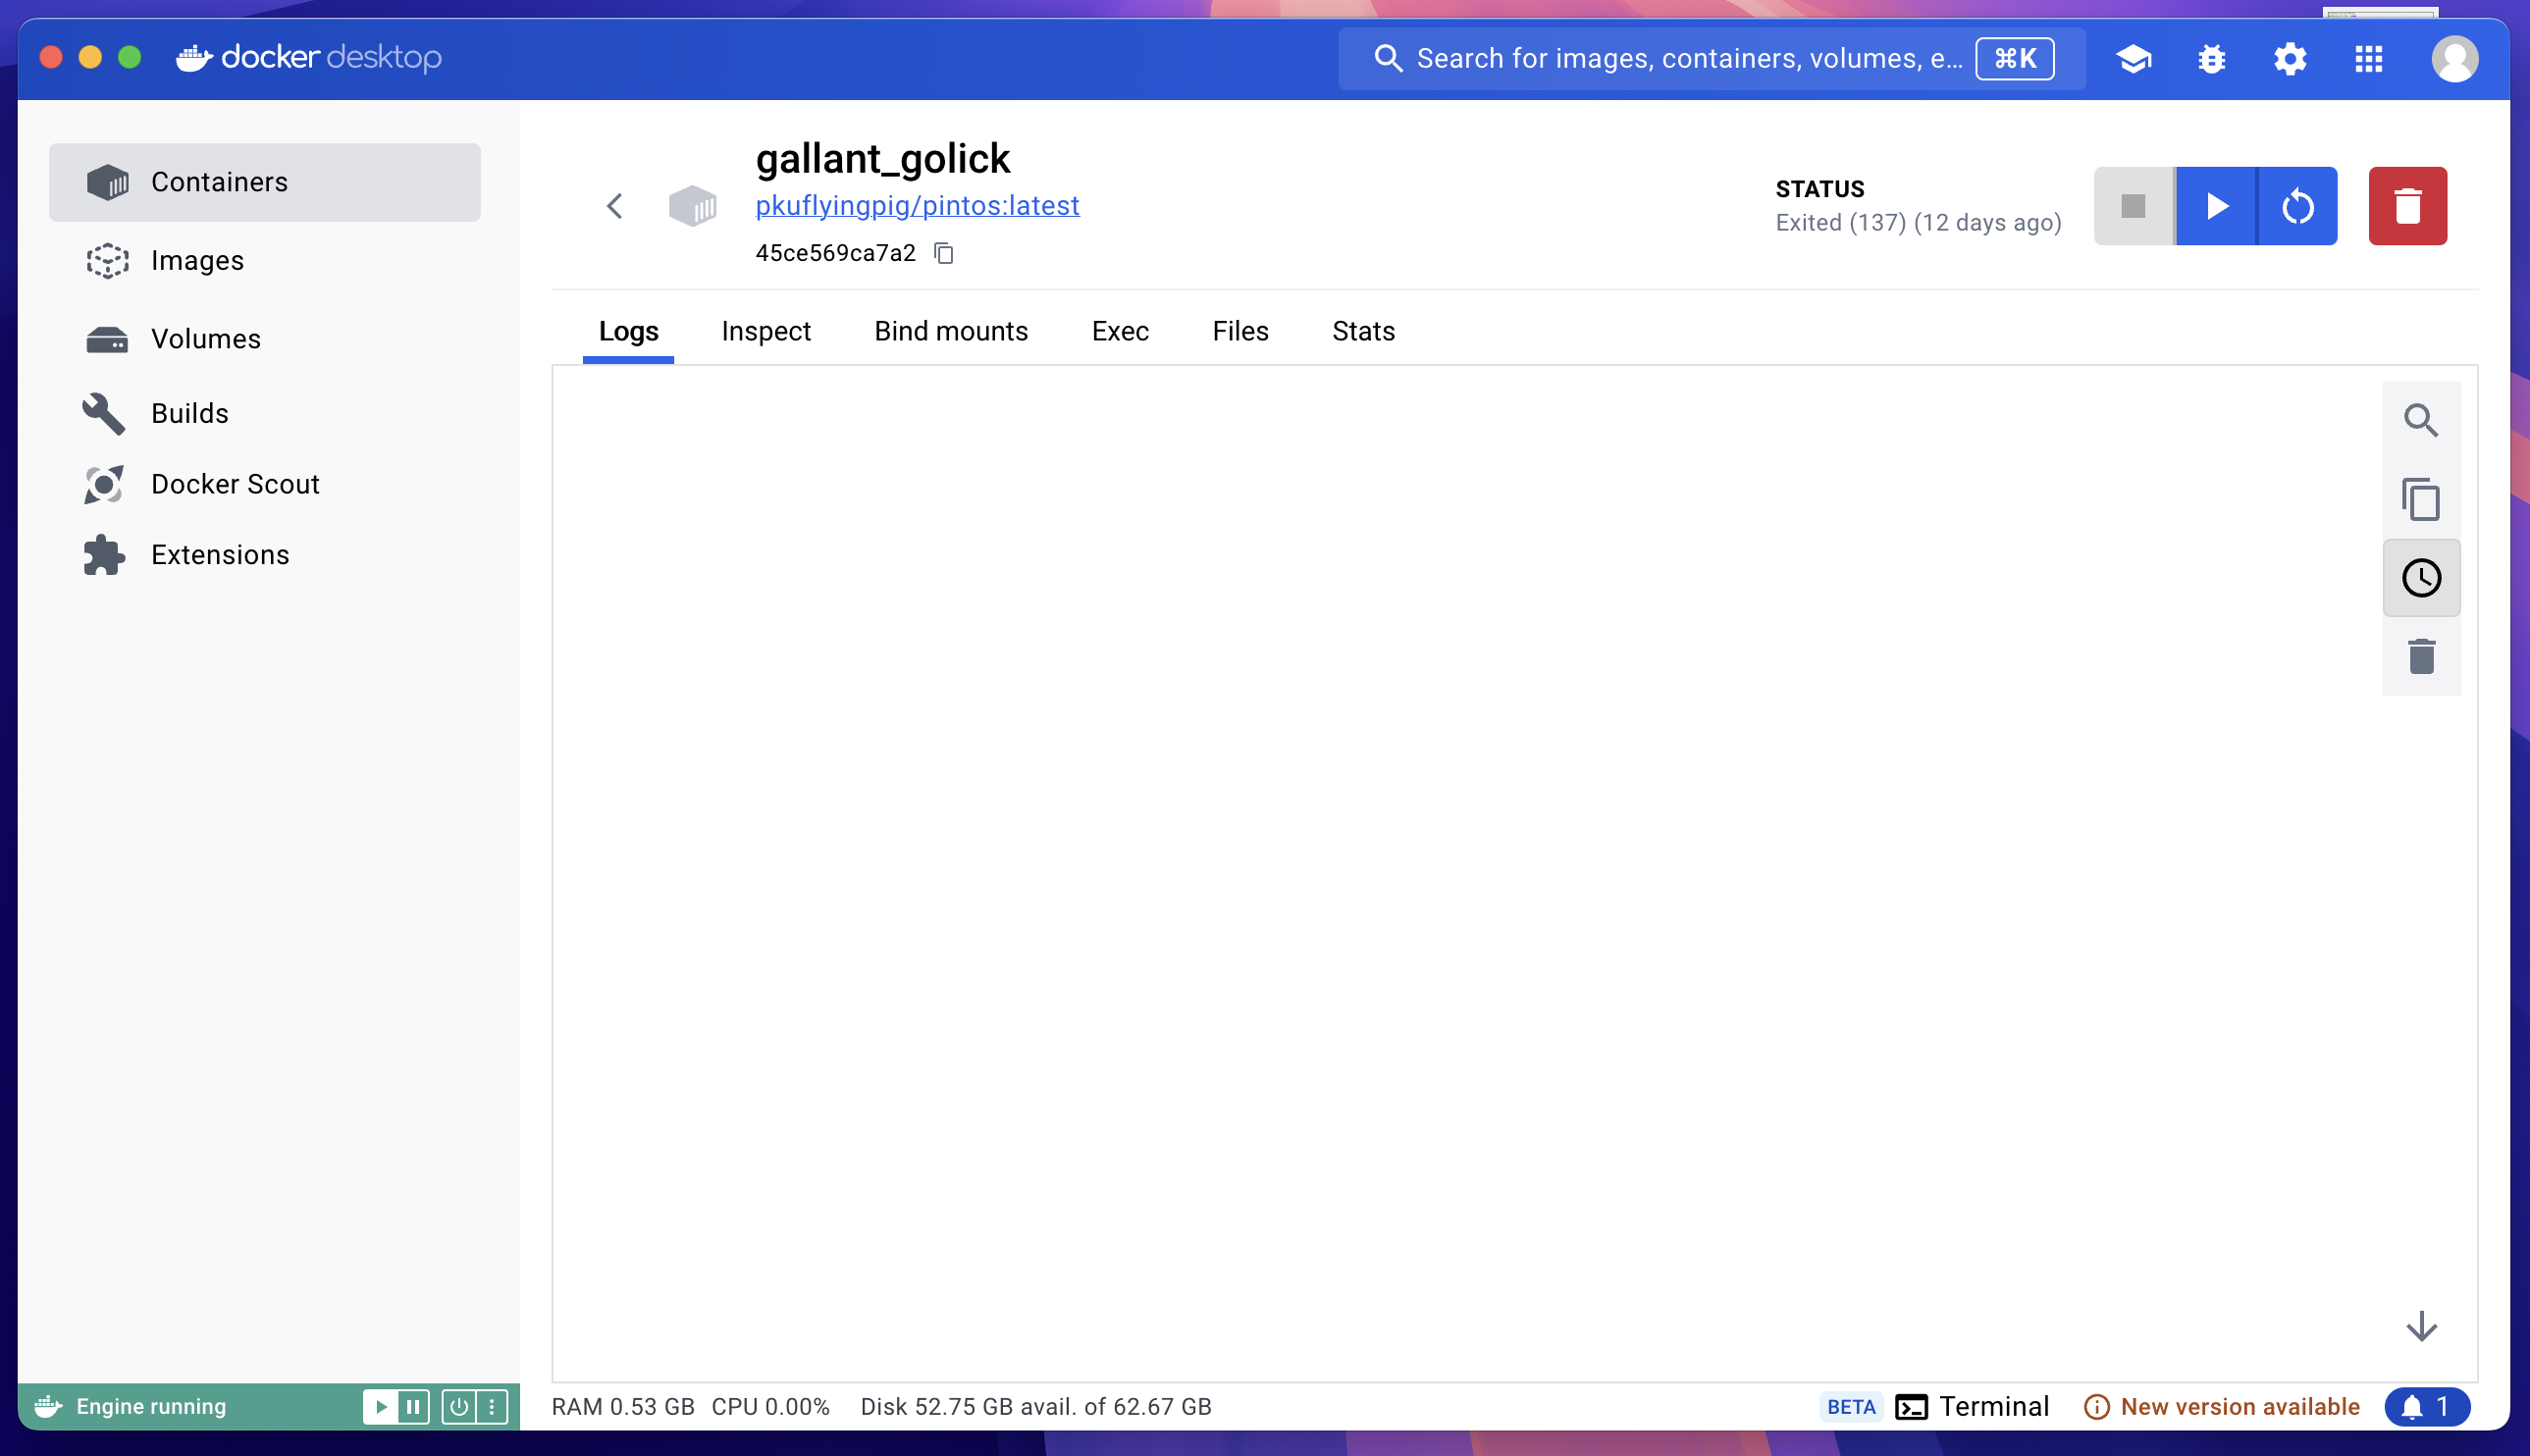
\includegraphics[width=0.9\textwidth]{img/docker_install.png}
	\caption{Docker容器}
\end{figure}

接着使用下面的命令实现磁盘挂载,方便文件管理:

\begin{lstlisting}[language=Bash, title=启动Docker容器并挂载文件]
	docker run -it --rm --name pintos --mount type=bind,source=/Users/wanghaisheng/Desktop/Coding/Courses/ECNU-Operating-System-WHS/pintos,target=/home/PKUOS/pintos pkuflyingpig/pintos bash
\end{lstlisting}

完成后如下图所示:

\begin{figure}[H]
	\centering
	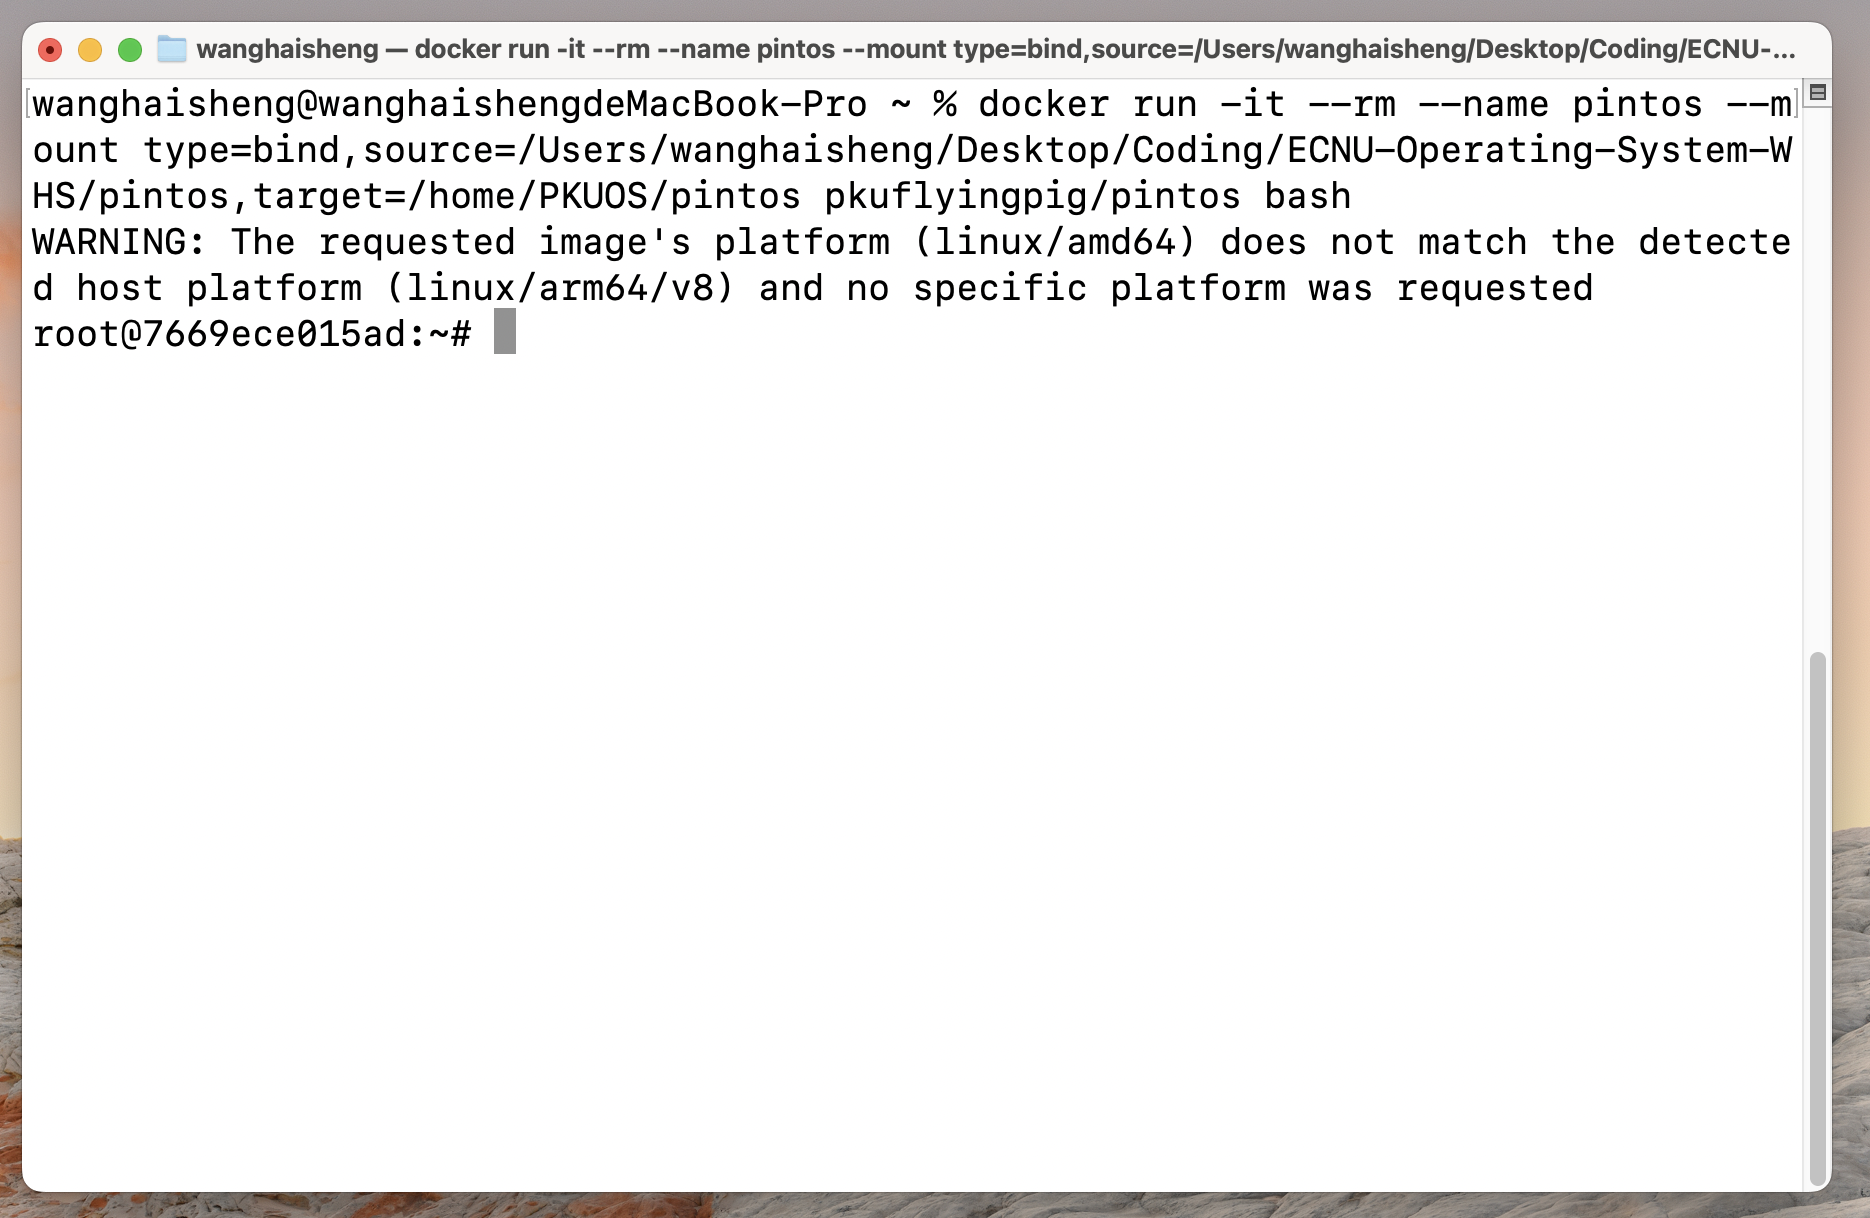
\includegraphics[width=0.9\textwidth]{img/run_docker.png}
	\caption{完成环境配置}
\end{figure}

\section{Accessing User Memory}

在用户使用系统调用时,可能会出现访问的地址超出用户可以访问的地址范围的情况,因此需要检查用户地址是否合法。对于整数类型,需要检查四个字节;对于字符串,则需要逐个字节进行检查。

根据文档说明,阅读 \texttt{userprog/pagedir.c} 和 \texttt{threads/vaddr.h} 文件可知,对于一个进程,用户可以访问的内存地址应在用户可访问的合理地址范围内,并且该地址必须已经映射为物理地址,即在页表中能找到对应的页。只有在满足这两个条件后,才能确认该地址是合法的。

\begin{lstlisting}[language=C]
	void *check_ptr(void *ptr, int byte)
	{
		int pd = thread_current()->pagedir;
		for (int i = 0; i < byte; i++)
		if (!is_user_vaddr(ptr + i) || pagedir_get_page(pd, ptr + i) == NULL)
		error_exit();
		return ptr;
	}
\end{lstlisting}

在之前的系统调用中加入指针检查后,\texttt{make\_check} 能够通过所有以 \texttt{sc} 开头的测试点。

\begin{lstlisting}[language=C]
	void syscall_exit(struct intr_frame *f)
	{
		int exit_code = *(int *)check_ptr(f->esp + 4, 4);
		thread_current()->exit_code = exit_code;
		thread_exit();
	}
	void syscall_wait(struct intr_frame *f)
	{
		int pid = *(int *)check_ptr(f->esp + 4, 4);
		f->eax = process_wait(pid);
	}
	void syscall_write(struct intr_frame *f)
	{
		int fd = *(int *)check_ptr(f->esp + 4, 4);
		char *buf = *(char **)check_ptr(f->esp + 8, 4);
		check_str(buf);
		int size = *(int *)check_ptr(f->esp + 12, 4);
		if (fd == 0)
		error_exit();
		if (fd == 1)
		{
			putbuf(buf, size);
			f->eax = size;
		}
	}
\end{lstlisting}

\begin{lstlisting}
	pass tests/userprog/sc-bad-sp
	pass tests/userprog/sc-bad-arg
	pass tests/userprog/sc-boundary
	pass tests/userprog/sc-boundary-2
	pass tests/userprog/sc-boundary-3
\end{lstlisting}

\section{Process System Call}

\subsection{halt \& exit}

根据文档,\texttt{halt} 直接调用了 \texttt{shutdown\_power\_off} 函数。需要注意的是,每个 \texttt{exit\_info} 的生命周期都比对应的进程生命周期长,因此与 \texttt{exit} 相关的错误码可以仅保存在每个进程的 \texttt{exit\_info} 中,从而避免冗余存储。请确保将所有 \texttt{thread\_current()->exit\_code} 替换为 \texttt{thread\_current()->linked\_exit->exit\_code},同时在 \texttt{process\_exit} 中不再需要传递错误码。

\begin{lstlisting}[language=C]
	void syscall_halt(struct intr_frame *f)
	{
		shutdown_power_off();
	}
	
	void syscall_exit(struct intr_frame *f)
	{
		int exit_code = *(int *)check_ptr(f->esp + 4, 4);
		thread_current()->linked_exit->exit_code = exit_code;
		thread_exit();
	}
\end{lstlisting}

\subsection{wait \& exec}

\texttt{wait} 函数在之前的实验中已经实现。根据 \texttt{exec} 函数的定义 \texttt{pid\_t exec (const char *cmd\_line)},该函数接收一个命令行字符串作为参数,并返回子进程的 \texttt{id}。如果子进程创建失败,则返回 \texttt{-1}。父进程需要等待子进程创建完成。

\begin{lstlisting}[language=C]
	void syscall_exec(struct intr_frame *f)
	{
		char *cmd = *(char **)check_ptr(f->esp + 4, 4);
		check_str(cmd);
		f->eax = process_execute(cmd);
	}
\end{lstlisting}

为实现同步,需要再定义一个 \texttt{sema\_exec},同时在 \texttt{init\_thread} 中进行初始化。然而,子进程无法通知父进程是否创建成功,因此使用一个 \texttt{exec\_success} 字段,让子进程修改以指示创建是否成功。

\begin{lstlisting}[language=C]
	struct thread
	{
		/* Owned by thread.c. */
		tid_t tid;    /** Thread identifier. */
		enum thread_status status;    /** Thread state. */
		char name[16];    /** Name (for debugging purposes). */
		uint8_t *stack;    /**< Saved stack pointer. */ 
		int priority;    /**< Priority. */ 
		struct list_elem allelem;    /**< List element for all threads list. */ 
		struct list_elem waitelem; 
		int64_t wake_tick; 
		/* Shared between thread.c and synch.c. */ 
		struct list_elem elem;    /**< List element. */ 
		#ifdef USERPROG 
		/* Owned by userprog/process.c. */ 
		uint32_t *pagedir;    /**< Page directory. */ 
		struct list child_list; 
		struct exit_info *linked_exit; 
		struct semaphore sema_wait; 
		struct semaphore sema_exec; 
		bool exec_success; 
		#endif 
		/* Owned by thread.c. */ 
		unsigned magic;    /**< Detects stack overflow. */ 
	};
	
	static void 
	init_thread (struct thread *t, const char *name, int priority) 
	{ 
		enum intr_level old_level; 
		ASSERT (t != NULL); 
		ASSERT (PRI_MIN <= priority && priority <= PRI_MAX); 
		ASSERT (name != NULL); 
		memset (t, 0, sizeof *t); 
		t->status = THREAD_BLOCKED; 
		strlcpy (t->name, name, sizeof t->name); 
		t->stack = (uint8_t *) t + PGSIZE; 
		t->priority = priority; 
		t->magic = THREAD_MAGIC; 
		t->wake_tick = -1; 
		list_init(&t->child_list); 
		sema_init(&t->sema_wait, 0); 
		sema_init(&t->sema_exec, 0); 
		old_level = intr_disable (); 
		list_insert_ordered(&all_list, &t->allelem, thread_more_priority, NULL); 
		intr_set_level (old_level); 
	}
\end{lstlisting}

在父进程的 \texttt{process\_execute} 中,调用 \texttt{thread\_create} 后,需要进行 P 操作以等待子进程完成创建。随后,父进程获取子进程的状态并返回。在子进程的 \texttt{start\_process} 中,管理好 \texttt{file\_name} 和 \texttt{cmd} 的生命周期后,填写父进程的 \texttt{exec\_success} 字段,接着进行 V 操作并退出。

\begin{lstlisting}[language=C]
	tid_t
	process_execute (const char *file_name)
	{
		char *fn_copy, *name_copy;
		tid_t tid;
		
		fn_copy = palloc_get_page(0);
		name_copy = palloc_get_page(0);
		if (fn_copy == NULL || name_copy == NULL)
		return TID_ERROR;
		
		strlcpy (fn_copy, file_name, PGSIZE);
		strlcpy (name_copy, file_name, PGSIZE);
		
		char *save_ptr;
		name_copy = strtok_r(name_copy, " ", &save_ptr);
		
		tid = thread_create (name_copy, PRI_DEFAULT, start_process, fn_copy);
		
		palloc_free_page(name_copy);
		
		if (tid == TID_ERROR)
		palloc_free_page (fn_copy);
		
		struct thread* cur = thread_current();
		sema_down(&cur->sema_exec);
		if (!cur->exec_success) return TID_ERROR;
		
		return tid;
	}
	
	static void
	start_process (void *file_name_)
	{
		char *file_name = file_name_; 
		struct intr_frame if_; 
		bool success;
		
		/* Initialize interrupt frame and load executable. */
		memset (&if_, 0, sizeof if_);
		if_.gs = if_.fs = if_.es = if_.ds = if_.ss = SEL_UDSEG;
		if_.cs = SEL_UCSEG;
		if_.eflags = FLAG_IF || FLAG_MBS;
		
		struct thread *cur = thread_current();
		
		char *cmd = palloc_get_page(0);
		if (cmd != NULL)
		{
			strlcpy(cmd, file_name_, PGSIZE);
			
			char *save_ptr;
			file_name = strtok_r(file_name, " ", &save_ptr);
			success = load (file_name, &if_.eip, &if_.esp);
			
			if (success)
			{
				push_argument(&if_.esp, cmd);
				palloc_free_page(cmd);
				palloc_free_page(file_name);
				
				cur->linked_exit->parent->exec_success = true;
				sema_up(&cur->linked_exit->parent->sema_exec);
				asm volatile ("movl %0, %%esp; jmp intr_exit" : : "g" (&if_) : "memory");
				NOT_REACHED ();
			}
			palloc_free_page(cmd);
		}
		
		palloc_free_page(file_name);
		cur->linked_exit->parent->exec_success = false;
		sema_up(&cur->linked_exit->parent->sema_exec);
		error_exit();
	}
\end{lstlisting}

至此可以通过 \texttt{exec} 和 \texttt{wait} 相关的测试点。

\begin{lstlisting}
	pass tests/userprog/exec-once
	pass tests/userprog/exec-arg
	pass tests/userprog/exec-bound
	pass tests/userprog/exec-bound-2
	pass tests/userprog/exec-bound-3
	pass tests/userprog/exec-multiple
	pass tests/userprog/exec-missing
	pass tests/userprog/exec-bad-ptr
	pass tests/userprog/wait-simple
	pass tests/userprog/wait-twice
	pass tests/userprog/wait-killed
	pass tests/userprog/wait-bad-pid
\end{lstlisting}

\section{File System Call}

根据文档描述,当前的文件系统是非线程安全的。因此,需要引入一个全局的文件锁来确保文件系统的互斥访问。具体实现如下:在 \texttt{thread.h} 中定义 \texttt{struct lock filesys\_lock},并在 \texttt{thread\_init} 函数中通过 \texttt{lock\_init(\&filesys\_lock)} 初始化该全局锁。在完善系统调用后,即可完成与 \texttt{create} 相关的测试点。

\subsection{create \& remove}

\begin{lstlisting}[language=C]
	void syscall_create(struct intr_frame *f)
	{
		char *file_name = *(char **)check_ptr(f->esp + 4, 4);
		check_str(file_name);
		int file_size = *(int *)check_ptr(f->esp + 8, 4);
		
		lock_acquire(&filesys_lock);
		f->eax = filesys_create(file_name, file_size);
		lock_release(&filesys_lock);
	}
	
	void syscall_remove(struct intr_frame *f)
	{
		char *file_name = *(char **)check_ptr(f->esp + 4, 4);
		check_str(file_name);
		
		lock_acquire(&filesys_lock);
		f->eax = filesys_remove(file_name);
		lock_release(&filesys_lock);
	}
\end{lstlisting}

\begin{lstlisting}
	pass tests/userprog/create-normal
	pass tests/userprog/create-empty
	pass tests/userprog/create-null
	pass tests/userprog/create-bad-ptr
	pass tests/userprog/create-long
	pass tests/userprog/create-exists
	pass tests/userprog/create-bound
\end{lstlisting}

\subsection{open \& close}

根据文档,每个进程需要维护其打开的文件信息。为此,需要在 \texttt{thread} 结构中新增一个文件列表,并维护文件的相关信息,如文件描述符和文件指针。在 \texttt{init\_thread} 函数中初始化该链表。同时,需要记录分配文件的下标,并将其初始化为 2,以避开标准输入输出 \texttt{buffer}。

\begin{lstlisting}[language=C]
	// struct thread 中
	#ifdef USERPROG
	/* Owned by userprog/process.c. */
	uint32_t *pagedir; /*< Page directory. */
	
	struct list child_list;
	struct exit_info *linked_exit;
	struct semaphore sema_wait;
	struct semaphore sema_exec;
	bool exec_success;
	
	struct list file_list;
	uint32_t file_index;
	
	#endif
	
	struct file_info
	{
		int fd;
		struct file* f;
		struct list_elem elem;
	};
\end{lstlisting}

为了对指定文件进行读写操作,需要在 \texttt{file\_list} 中找到相应的文件,实现辅助函数来遍历链表。

\begin{lstlisting}[language=C]
	struct file_info *foreach_file(int fd)
	{
		struct thread* cur = thread_current();
		struct list * l = &cur->file_list;
		struct list_elem *e;
		
		for (e = list_begin(l); e != list_end(l); e = list_next(e)) { 
			struct file_info* tmp = list_entry(e, struct file_info, elem); 
			if (tmp->fd == fd) return tmp; 
		} 
		return NULL; 
	}
\end{lstlisting}

此时可以实现系统调用。打开文件时,将文件初始化并插入链表;关闭文件时,将其从链表中删除并释放内存。最后在 \texttt{process\_exit} 时释放所有打开的文件。

\begin{lstlisting}[language=C]
	while (!list_empty(&cur->file_list)) { 
		e = list_pop_front(&cur->file_list); 
		struct file_info* tmp = list_entry(e, struct file_info, elem); 
		lock_acquire(&filesys_lock); 
		file_close(tmp->f); 
		lock_release(&filesys_lock); 
		free(tmp); 
	}
	
	void syscall_open(struct intr_frame *f) { 
		char *file_name = *(char **)check_ptr(f->esp + 4, 4); 
		check_str(file_name);
		
		lock_acquire(&filesys_lock); 
		struct file* open_file = filesys_open(file_name); 
		lock_release(&filesys_lock);
		
		if (open_file == NULL) { 
			f->eax = -1; 
			return; 
		}
		
		struct thread *cur = thread_current(); 
		struct file_info *tmp = malloc(sizeof(struct file_info)); 
		tmp->f = open_file; 
		tmp->fd = cur->file_index++; 
		list_push_back(&cur->file_list, &tmp->elem); 
		f->eax = tmp->fd; 
	}
	
	void syscall_close(struct intr_frame *f) { 
		int fd = *(int *)check_ptr(f->esp + 4, 4);
		
		struct file_info* tmp = foreach_file(fd); 
		if (tmp != NULL) { 
			lock_acquire(&filesys_lock); 
			file_close(tmp->f); 
			list_remove(&tmp->elem); 
			free(tmp); 
			lock_release(&filesys_lock); 
		}
	}
\end{lstlisting}

此时可以通过\texttt{open}和\texttt{close}相关的测试点。

\begin{lstlisting}
	pass tests/userprog/open-null
	pass tests/userprog/open-bad-ptr
	pass tests/userprog/open-twice
	pass tests/userprog/close-normal
	pass tests/userprog/close-twice
	pass tests/userprog/close-stdin
	pass tests/userprog/close-stdout
	pass tests/userprog/close-bad-fd
\end{lstlisting}

\subsection{read \& write \& filesize}

由于 \texttt{read} 和 \texttt{write} 的测试需要调用 \texttt{filesize} 系统调用,因此在此处也需要实现 \texttt{filesize}。直接根据文档调用文件系统的 API 即可,但不要忘记加锁。此外,还需要注意将 \texttt{src/tests/vm/sample.txt} 和 \texttt{src/tests/userprog/sample.txt} 文件的行尾序列改为 LF。完成这些后,即可通过 \texttt{read} 和 \texttt{write} 相关的测试点。

\begin{lstlisting}[language=C]
	void syscall_read(struct intr_frame *f)
	{
		int fd = *(int *)check_ptr(f->esp + 4, 4);
		char *buf = *(char **)check_ptr(f->esp + 8, 4);
		check_str(buf);
		int size = *(int *)check_ptr(f->esp + 12, 4);
		
		if (fd == 1) error_exit();
		if (fd == 0)
		{
			for (int i = 0; i < size; i++)
			*buf = input_getc(), buf++;
			f->eax = size;
		}
		else
		{
			struct file_info* tmp = foreach_file(fd);
			if (tmp == NULL) f->eax = -1;
			else
			{
				lock_acquire(&filesys_lock);
				f->eax = file_read(tmp->f, buf, size);
				lock_release(&filesys_lock);
			}
		}
	}
	
	void syscall_write(struct intr_frame *f)
	{
		int fd = *(int *)check_ptr(f->esp + 4, 4);
		char *buf = *(char **)check_ptr(f->esp + 8, 4);
		check_str(buf);
		int size = *(int *)check_ptr(f->esp + 12, 4);
		
		if (fd == 0) error_exit();
		if (fd == 1)
		{
			putbuf(buf, size);
			f->eax = size;
		}
		else
		{
			struct file_info* tmp = foreach_file(fd);
			if (tmp == NULL) f->eax = -1;
			else
			{
				lock_acquire(&filesys_lock);
				f->eax = file_write(tmp->f, buf, size);
				lock_release(&filesys_lock);
			}
		}
	}
	
	void syscall_filesize(struct intr_frame *f)
	{
		int fd = *(int *)check_ptr(f->esp + 4, 4);
		struct file_info* tmp = foreach_file(fd);
		if (tmp->f == NULL) f->eax = -1;
		else
		{
			lock_acquire(&filesys_lock);
			f->eax = file_length(tmp->f);
			lock_release(&filesys_lock);
		}
	}
\end{lstlisting}

\begin{lstlisting}
	pass tests/userprog/read-normal
	pass tests/userprog/read-bad-ptr
	pass tests/userprog/read-boundary
	pass tests/userprog/read-zero
	pass tests/userprog/read-stdout
	pass tests/userprog/read-bad-fd
	pass tests/userprog/write-normal
	pass tests/userprog/write-bad-ptr
	pass tests/userprog/write-boundary
	pass tests/userprog/write-zero
	pass tests/userprog/write-stdin
	pass tests/userprog/write-bad-fd
\end{lstlisting}	

\subsection{seek \& tell}

同样根据文档实现,直接调用文件系统的\texttt{api}。

\begin{lstlisting}[language=C]
	void syscall_seek(struct intr_frame * f)
	{
		int fd = *(int *)check_ptr(f->esp + 4, 4);
		int pos = *(int *)check_ptr(f->esp + 8, 4);
		struct file_info* tmp = foreach_file(fd);
		if (tmp != NULL)
		{
			lock_acquire(&filesys_lock);
			file_seek(tmp->f, pos);
			lock_release(&filesys_lock);
		}
	}
	
	void syscall_tell(struct intr_frame *f)
	{
		int fd = *(int *)check_ptr(f->esp + 4, 4);
		struct file_info* tmp = foreach_file(fd);
		if (tmp != NULL)
		{
			lock_acquire(&filesys_lock);
			f->eax = file_tell(tmp->f);
			lock_release(&filesys_lock);
		}
		else f->eax = -1;
	}
\end{lstlisting}

自此,除了\texttt{rox}相关的测试点,其他全部通过。

\begin{lstlisting}
	FAIL tests/userprog/rox-simple
	FAIL tests/userprog/rox-child
	FAIL tests/userprog/rox-multichild
\end{lstlisting}

\section{Denying Writes to Executables}

在程序运行时,拒绝其他程序对其进行写入操作。在 \texttt{thread} 中记录当前运行的文件 \texttt{exec\_file},注意初始化为 \texttt{NULL}。按照文档要求,在加载程序文件前后获取和释放锁。读文件成功后,调用 \texttt{file\_deny\_write} 并更新 \texttt{exec\_file}。在 \texttt{thread\_exit} 的结尾,判断如果 \texttt{exec\_file} 不为空,则调用 \texttt{file\_allow\_write} 并关闭文件。

\begin{lstlisting}[language=C]
	// start process
	lock_acquire(&filesys_lock);
	success = load (file_name, &if_.eip, &if_.esp);
	if (success)
	{
		struct file *f = filesys_open(file_name);
		cur->exec_file = f;
		file_deny_write(f);
	}
	lock_release(&filesys_lock);
	
	// thread_exit
	if (cur->exec_file != NULL)
	{
		lock_acquire(&filesys_lock);
		file_allow_write(cur->exec_file);
		file_close(cur->exec_file);
		lock_release(&filesys_lock);
	}
\end{lstlisting}

\section{实验结果:\texttt{make check}全部通过}

至此,\texttt{make check}中的测试点全部通过。

\begin{lstlisting}
	pass tests/userprog/args-none
	pass tests/userprog/args-single
	pass tests/userprog/args-multiple
	pass tests/userprog/args-many
	pass tests/userprog/args-dbl-space
	pass tests/userprog/sc-bad-sp
	pass tests/userprog/sc-bad-arg
	pass tests/userprog/sc-boundary
	pass tests/userprog/sc-boundary-2
	pass tests/userprog/sc-boundary-3
	pass tests/userprog/halt
	pass tests/userprog/exit
	pass tests/userprog/create-normal
	pass tests/userprog/create-empty
	pass tests/userprog/create-null
	pass tests/userprog/create-bad-ptr
	pass tests/userprog/create-long
	pass tests/userprog/create-exists
	pass tests/userprog/create-bound
	pass tests/userprog/open-normal
	pass tests/userprog/open-missing
	pass tests/userprog/open-boundary
	pass tests/userprog/open-empty
	pass tests/userprog/open-null
	pass tests/userprog/open-bad-ptr
	pass tests/userprog/open-twice
	pass tests/userprog/close-normal
	pass tests/userprog/close-twice
	pass tests/userprog/close-stdin
	pass tests/userprog/close-stdout
	pass tests/userprog/close-bad-fd
	pass tests/userprog/read-normal
	pass tests/userprog/read-bad-ptr
	pass tests/userprog/read-boundary
	pass tests/userprog/read-zero
	pass tests/userprog/read-stdout
	pass tests/userprog/read-bad-fd
	pass tests/userprog/write-normal
	pass tests/userprog/write-bad-ptr
	pass tests/userprog/write-boundary
	pass tests/userprog/write-zero
	pass tests/userprog/write-stdin
	pass tests/userprog/write-bad-fd
	pass tests/userprog/exec-once
	pass tests/userprog/exec-arg
	pass tests/userprog/exec-bound
	pass tests/userprog/exec-bound-2
	pass tests/userprog/exec-bound-3
	pass tests/userprog/exec-multiple
	pass tests/userprog/exec-missing
	pass tests/userprog/exec-bad-ptr
	pass tests/userprog/wait-simple
	pass tests/userprog/wait-twice
	pass tests/userprog/wait-killed
	pass tests/userprog/wait-bad-pid
	pass tests/userprog/multi-recurse
	pass tests/userprog/multi-child-fd
	pass tests/userprog/rox-simple
	pass tests/userprog/rox-child
	pass tests/userprog/rox-multichild
	pass tests/userprog/bad-read
	pass tests/userprog/bad-write
	pass tests/userprog/bad-read2
	pass tests/userprog/bad-write2
	pass tests/userprog/bad-jump
	pass tests/userprog/bad-jump2
	pass tests/userprog/no-vm/multi-oom
	pass tests/filesys/base/lg-create
	pass tests/filesys/base/lg-full
	pass tests/filesys/base/lg-random
	pass tests/filesys/base/lg-seq-block
	pass tests/filesys/base/lg-seq-random
	pass tests/filesys/base/sm-create
	pass tests/filesys/base/sm-full
	pass tests/filesys/base/sm-random
	pass tests/filesys/base/sm-seq-block
	pass tests/filesys/base/sm-seq-random
	pass tests/filesys/base/syn-read
	pass tests/filesys/base/syn-remove
	pass tests/filesys/base/syn-write
	All 80 tests passed.
	make[1]: Leaving directory /Users/wanghaisheng/Desktop/Coding/Courses/ECNU-Operating-System-WHS/pintos/src/userprog/build
\end{lstlisting}

\section{实验总结}

通过本次实验,我深入理解了操作系统中的系统调用机制,并成功实现了\texttt{Pintos}中的一系列系统调用功能,通过了\texttt{make check}中的全部测试点。在实验过程中,我不仅掌握了如何从用户态切换到内核态、传递参数和返回结果的基本流程,还学会了如何处理进程同步和文件系统的线程安全问题。特别是在实现文件操作系统调用时,我遇到了多个并发访问的挑战,通过引入全局锁和合理的内存管理,最终确保了系统的稳定性和正确性。

\end{document}